\documentclass[11pt,sigconf]{iabart}
%\documentclass[10pt,sigconf,letterpaper]{acmart}
%\usepackage[vskip=1em,font=itshape,leftmargin=2em,rightmargin=2em]{quoting}
\usepackage[skip=4pt plus1pt]{parskip}
%\copyrightyear{2024}
%\acmYear{2024}
%\setcopyright{acmlicensed}\acmConference[IAB Network Management WS]{The IAB Next Era of Network Management Operations}{December 3, 2024}{}
%\acmBooktitle{The IAB next Era of Network Management Workshop}{December 3, 2024}{}

\begin{document}

\title{LwM2M TITLE WIP}

\author{Jaime Jiménez}
\email{jaime.jimenez@ericsson.com}
\orcid{0009-0008-2864-4269}
\affiliation{%
  \institution{Ericsson}
  \city{Jorvas}
  \country{Finland}
}
\author{Matthew Gillmore}
\email{email@email}
\orcid{orcidID}
\affiliation{%
  \institution{Itron}
  \city{City}
  \country{Country}
}

\begin{abstract}
%Jaime: Write a concise abstract (150-250 words) summarizing the paper's purpose, methods, key findings, and implications.
TBD.

\end{abstract}

\keywords{IoT, network management, LwM2M, device management, protocol, scalability, security}

\maketitle

\section{Introduction} \label{introduction}


%Jaime: We need to address gaps, such as operator-specific challenges or more detailed recommendations for future standardization efforts.

The rapid evolution of network management protocols necessitates a reevaluation of existing technologies and their applicability to modern challenges. The Lightweight Machine-to-Machine (LwM2M) protocol~\cite{lwm2m-spec}, developed by the Open Mobile Alliance (OMA), is a key player in this domain, offering a standardized framework for managing Internet of Things (IoT) devices~\cite{oma-sdo}. This paper explores the role of LwM2M in the context of the IAB workshop on the Next Era of Network Management Operations, focusing on its current deployments, challenges, and future potential.

The IAB "NEMOPS" workshop seeks contributions that critically assess the progress made since the 2002 IAB workshop, particularly in terms of network management protocols. This paper aims to present LwM2M's as a new protocol created after 2002 that addresses the needs for managing IoT endpoints from the operational point of view of device and network management.

Our contribution is informed by the authors' extensive experience with IoT and contributions in the IoT domain both at IETF and in OMA. The rest of the document is organized as follows: The \hyperref[introduction]{Introduction} outlines LwM2M as a standardized framework for managing IoT devices, addressing current network management challenges. The \hyperref[overview]{LwM2M Protocol Overview} details its architecture, focusing on communication between Clients, Servers, and Bootstrap Servers (see Figure~\ref{fig:overall_architecture}). Recent advancements, including integrations with blockchain and industrial protocols, are discussed in \hyperref[extensions]{LwM2M Extensions}, highlighting its adaptability. Remaining adoption challenges are explored in \hyperref[operations]{LwM2M Operations}, while the \hyperref[conclusions]{Conclusions} summarize key findings and future directions.

\textbf{LwM2M and IETF}

The IETF has played a fundamental role in shaping the protocols that underpin Lightweight Machine-to-Machine (LwM2M). IETF efforts have fcused on adapting existing Internet and Web protocols to meet the needs of resource-constrained IoT devices ~\cite{9139045}. These protocols enable efficient communication, security, and interoperability, forming a foundation for LwM2M.

The Lightweight Machine-to-Machine (LwM2M) protocol is built upon several key IETF standards. At the core is the \textit{Constrained Application Protocol (CoAP)}~\cite{rfc7252}, a lightweight RESTful protocol designed for constrained environments, providing the fundamental request/ response model for LwM2M communications. CoAP supports features such as observe/notify, which are critical for resource updates. Additionally, \textit{RFC 7959}~\cite{rfc7959} defines block-wise transfers in CoAP, allowing LwM2M to efficiently handle large payloads by breaking them into smaller blocks. The \textit{LwM2M} protocol also leverages \textit{RFC 7641}~\cite{rfc7641} for resource observation, enabling clients to monitor changes to resources without continuous polling. For secure communications, LwM2M often relies on the \textit{Datagram Transport Layer Security (DTLS)} as outlined in \textit{RFC 6347}~\cite{rfc6347}, ensuring encryption and integrity over the CoAP protocol. An additional layer of security is provided by \textit{Object Security for Constrained RESTful Environments (OSCORE)}~\cite{rfc8613}, which offers end-to-end encryption and integrity protection directly at the application layer, making it suitable for scenarios where DTLS is not applicable. 


Furthermore, LwM2M also supports other transport protocols such as \textit{MQTT}~\cite{mqtt-spec} and \textit{HTTP}~\cite{http-spec}, broadening its applicability across different network environments and use cases.

\section{LwM2M Protocol Overview} \label{overview}

\begin{figure}[h]
  \centering
  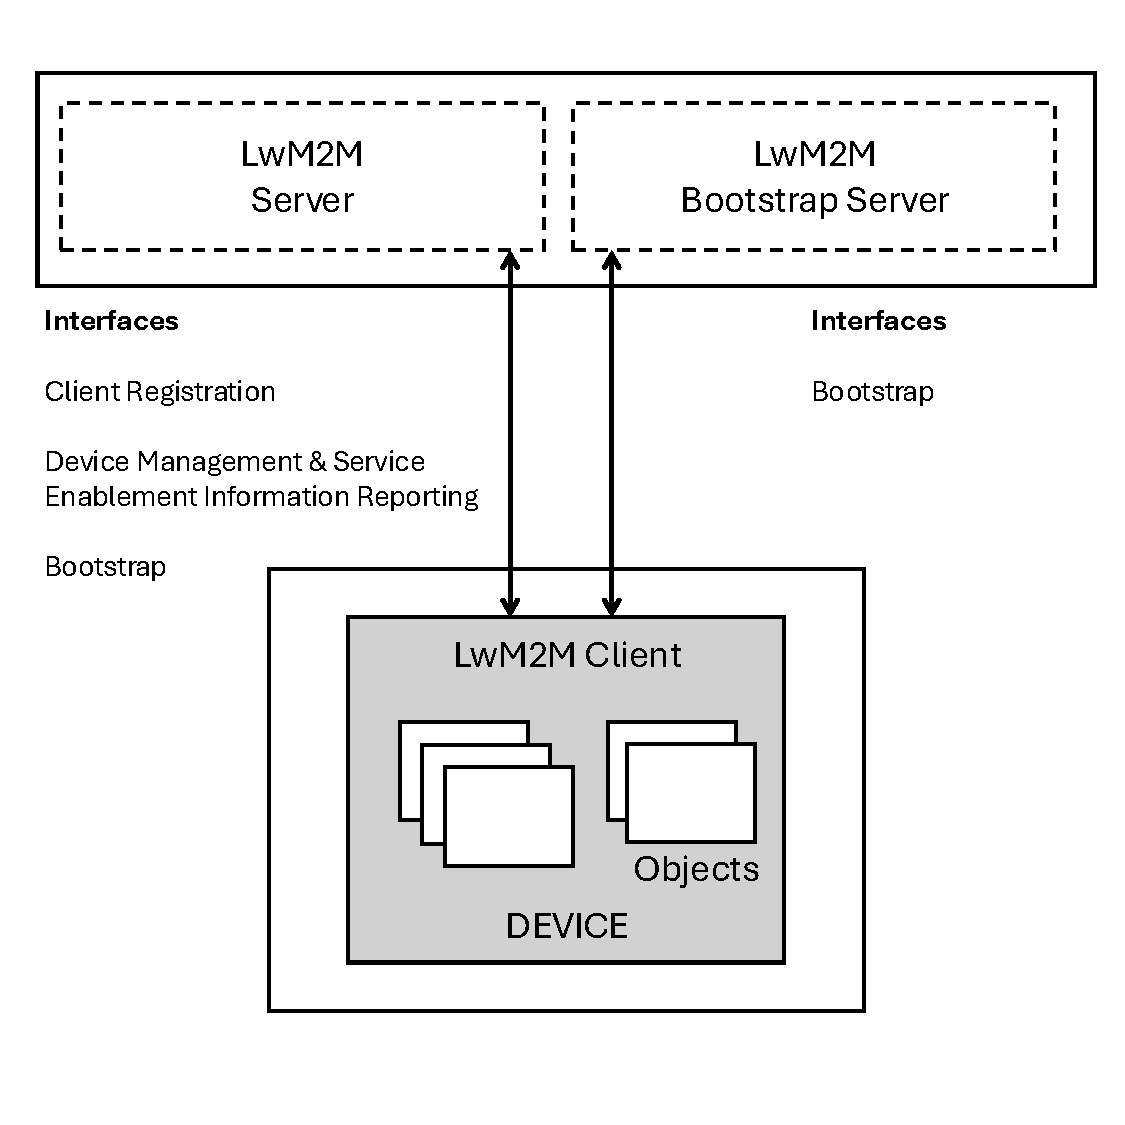
\includegraphics[width=0.5\textwidth]{figs/arch.pdf}
  \caption{General LwM2M Architecture}
  \label{fig:overall_architecture}
\end{figure}

This section presents an overview of the LwM2M protocol, emphasizing its participating entities, data model, and communication interfaces. Additionally, it describes the LwM2M library's design and functionality, highlighting challenges encountered during its development.

\textbf{Participating Entities}

The LwM2M protocol defines three primary entities that form the backbone of its communication architecture:
\begin{itemize}
    \item \textbf{LwM2M Client}: This entity is typically a device responsible for data collection and managing resources, such as sensors or other IoT devices. The client manages the lifecycle of various objects and interacts with servers to share collected data and receive management commands.
    \item \textbf{LwM2M Server}: This server is responsible for managing multiple clients, aggregating their data, and issuing commands for configuration or maintenance. It plays a crucial role in the control and coordination of client devices within an IoT ecosystem.
    \item \textbf{LwM2M Bootstrap Server}: This unique entity is tasked with the initial configuration of the LwM2M Client. Unlike other protocols, LwM2M introduces the Bootstrap Server to facilitate the initial setup of devices, especially when multiple servers are involved. During the bootstrap process, the Bootstrap Server provides the client with configuration details, such as security credentials and connection information, which can either be pre-integrated into the device's software or dynamically provided by the Bootstrap Server \cite{pop00006}.
\end{itemize}

The introduction of the Bootstrap Server differentiates LwM2M from other IoT protocols. Before the client can establish a connection to a server, it undergoes the bootstrap procedure to load initial configurations. This feature is particularly advantageous in scenarios with multiple servers or when load balancing is required, as it allows for flexible and dynamic configuration \cite{pop00006}.

\textbf{LwM2M Data Model}

The LwM2M protocol utilizes a structured, object-based data model, which simplifies communication between clients and servers. Each data entity in the LwM2M model is defined as an object, identified by a unique integer ID, as specified by the Open Mobile Alliance (OMA). These objects can represent various resources such as sensors, actuators, or configuration settings.

Each object comprises multiple resources, which are the fundamental data points within the object. Resources are also assigned integer IDs and are categorized as mandatory or optional based on the object's intended use. In some cases, an object can have multiple instances, each with a unique instance ID. This flexibility allows for scenarios where, for example, a device might have several temperature sensors, each represented as an instance of the same object \cite{pop00006}.

The LwM2M data model enables servers to access individual resources, instances, or entire objects using well-defined URI strings. The format of these URIs is as follows:
\[
/<Object ID>/<Instance ID>/<Resource ID>
\]
In this structure, the instance or resource ID can be omitted if the request targets the entire object or a specific instance. This model provides a straightforward way to interact with data at different levels of granularity.

\textbf{Communication Interfaces}

LwM2M defines four primary communication interfaces that facilitate interactions between clients and servers, each serving distinct roles in the protocol's operation:

\begin{itemize}
    \item \textbf{Bootstrap Interface}: This interface manages the bootstrap procedure, allowing the client to acquire initial configurations and security credentials from the Bootstrap Server before connecting to an LwM2M Server. The process can be automated or initiated by the client as needed.
    \item \textbf{Registration Interface}: After the bootstrap procedure, the client registers with the LwM2M Server through the Registration Interface. During registration, the client provides its endpoint name, which acts as an access token. The server can deny access if the provided token is invalid. To maintain its registration status, the client must periodically send updates. If these updates are not received within the agreed time, the client is considered de-registered and must re-initiate the registration process \cite{pop00006}.
    \item \textbf{Device Management and Service Enablement Interface}: Once registered, the server can use this interface to perform various management tasks, such as reading and writing data or executing commands on the client. It allows the server to control the client's resources, adjusting settings or triggering actions as required.
    \item \textbf{Information Reporting Interface}: This interface enables the client to report changes in its status or resource values to the server, using the Observe function. The server can set up observation requests, prompting the client to notify it when certain resource values change or when predefined conditions are met. This capability is particularly useful for monitoring dynamic IoT environments where timely updates are crucial. LwM2M defines specific attributes to configure how frequently these notifications occur \cite{pop00006}.
\end{itemize}

LwM2M has been integrated on most IoT OSs like Mbed~\cite{mbed}, RIOT OS~\cite{riot_os}, Contiki-NG~\cite{contiki_ng}, and others, with a strong focus on IoT device security~\cite{pop00010}.

\section{LwM2M Extensions} \label{extensions}

LwM2M, while robust in its core functionalities, has seen significant advancements through various extensions and integrations. This section delves into the recent developments and integrations of LwM2M, highlighting its evolving role in the IoT ecosystem.

\subsection{LwM2M Integrations}


%Jaime: Expand on the implications of these integrations for the future of IoT and network management.
The integration of LwM2M with other technologies has been researched, aiming to enhance the capabilities and interoperability of IoT systems. 

To name a few, Kim et al.~\cite{pop00007} designed and implemented a blockchain-based system that enables interworking between oneM2M and LwM2M IoT systems. This approach not only improves interoperability between different IoT frameworks but also enhances security by leveraging blockchain's immutable and distributed ledger properties. 

In the context of Industrial IoT (IIoT), Yaker et al.~\cite{pop00004} introduced a novel edge Security Information and Event Management (SIEM) system for managing IoT flows within 5G private networks. Their approach incorporates LwM2M data events, demonstrating how edge computing can effectively manage and secure IoT data in a 5G environment. Similarly, Myoung et al.~\cite{pop00012} addressed the integration of LwM2M with smart metering technologies, proposing a data interworking model between the Device Language Message Specification (DLMS)~\cite{dlms-spec} nd LwM2M protocols. Their work highlights the potential for harmonizing different IoT protocols within Advanced Metering Infrastructure (AMI) systems, thereby enabling more efficient data exchange and management.

Further efforts have been made to integrate LwM2M with industrial communication protocols. Karaagac et al.~\cite{pop00013} explored the interoperability between LwM2M and OPC UA (Open Platform Communications Unified Architecture), proposing a framework where OPC UA Servers can be virtualized as LwM2M Clients and vice versa. This approach aims to bridge the gap between IoT and industrial automation, facilitating seamless communication across heterogeneous systems. Similarly, Cavalcanti et al.~\cite{pop00014} reviewed various machine-to-machine communication protocols within the context of Industry 4.0, emphasizing the advantages of integrating OPC UA with LwM2M for industrial applications.

A last example, Wang et al.~\cite{pop00015} proposed a CoAP-based OPC UA transmission scheme tailored for resource-constrained devices. Although their work does not directly involve LwM2M, it illustrates the broader trend of adapting industrial communication protocols to fit the needs of IoT environments. Such efforts are indicative of a growing interest in enabling resource-efficient and interoperable solutions in the IoT landscape, especially where industrial and IoT domains converge.

The integration of LwM2M with these diverse technologies underscores its versatility and adaptability, positioning it as a critical component in the evolving IoT ecosystem.

\subsection{ Adoption of LwM2M in IoT Security}

The Lightweight Machine-to-Machine (LwM2M) protocol has emerged as a critical focus in recent IoT research, particularly concerning security improvements, implementation strategies, and integration with other technologies. This increased attention highlights its growing importance in advancing IoT systems.

Several studies have concentrated on enhancing IoT security through the use of LwM2M. For instance, Muhammad et al.~\cite{pop00001} investigated the use of ARIA cryptography within Hardware Secure Modules for both LwM2M and MQTT protocols, aiming to bolster the security of next-generation IoT systems. Similarly, Lanzieri et al.~\cite{pop00011} proposed extensions to the LwM2M core specification to facilitate secure and authorized client-to-client communication, thereby addressing a significant limitation of the standard protocol.

However, despite its promising capabilities, LwM2M still faces challenges in widespread adoption. Szydlo and Nagy~\cite{pop00003} pointed out the low market uptake of LwM2M in IoT products, attributing this to a lack of freely available developer tools. This observation underscores the need for more accessible resources to facilitate LwM2M implementation.

In parallel, Saif and Matrawy~\cite{pop00005} proposed and evaluated methods for the mass configuration of heterogeneous IIoT nodes using LwM2M, demonstrating potential solutions for scaling the protocol in diverse environments.

\section{LwM2M Operations} \label{operations}
%Jaime: Develop this section to cover typical operations, challenges, and best practices. Include examples of common operations and how they're implemented.
%Jaime: Add more specific examples of how LwM2M is used in real-world applications.



TBD


\section{Conclusions} \label{conclusions}

TBD

\section{Acknowledgments}

We'd like to thank Ericsson for their support of this work. We also appreciate A, B, C for their valuable discussions on this topic.

\bibliographystyle{ACM-Reference-Format}
\bibliography{paper}

\end{document}
\endinput
